\documentclass[9pt]{beamer}


\usepackage[LGR,T1]{fontenc}
\usepackage[utf8]{inputenc} 
\usepackage{color}
\usepackage{graphicx}
\usepackage{natbib}
\usepackage{tikz}
\usepackage{pgfgantt}
\usepackage{booktabs}
\usepackage{framed}

\usetheme{Boadilla}

\definecolor{rd}{HTML}{2F2A40}
\definecolor{methods}{HTML}{C6C6C6}
\definecolor{research}{HTML}{8F84BE}
\definecolor{skills}{HTML}{7A7A7A}
\definecolor{rc}{HTML}{AC152A} 

\newcommand{\textgreek}[1]{\begingroup\fontencoding{LGR}\selectfont#1\endgroup}

\usefonttheme{professionalfonts}

\title[Climate Topography]{A Topography of Climate Change Research}
\subtitle{}
\author{Max Callaghan}
\institute[MCC]{
	
\includegraphics[height=1cm,width=2cm]{MCC_Logo_RZ_rgb.jpg}
%	\,
%	
\includegraphics[height=1cm]{hertie_logo.png}
}

\newtheorem*{remark}{}

\bibliographystyle{apalike}

\begin{document}
	
\begin{frame}
	\titlepage
\end{frame}

\addtobeamertemplate{frametitle}{}{%
	\begin{tikzpicture}[remember picture,overlay]
	\node[anchor=north east,yshift=2pt] at (current page.north east) {
\includegraphics[height=0.8cm]{MCC_Logo_RZ_rgb.jpg}};
	\end{tikzpicture}}

\begin{frame}{Introduction}
\begin{columns}
	\begin{column}{0.6\linewidth}
		\begin{center}
			\begin{figure}
			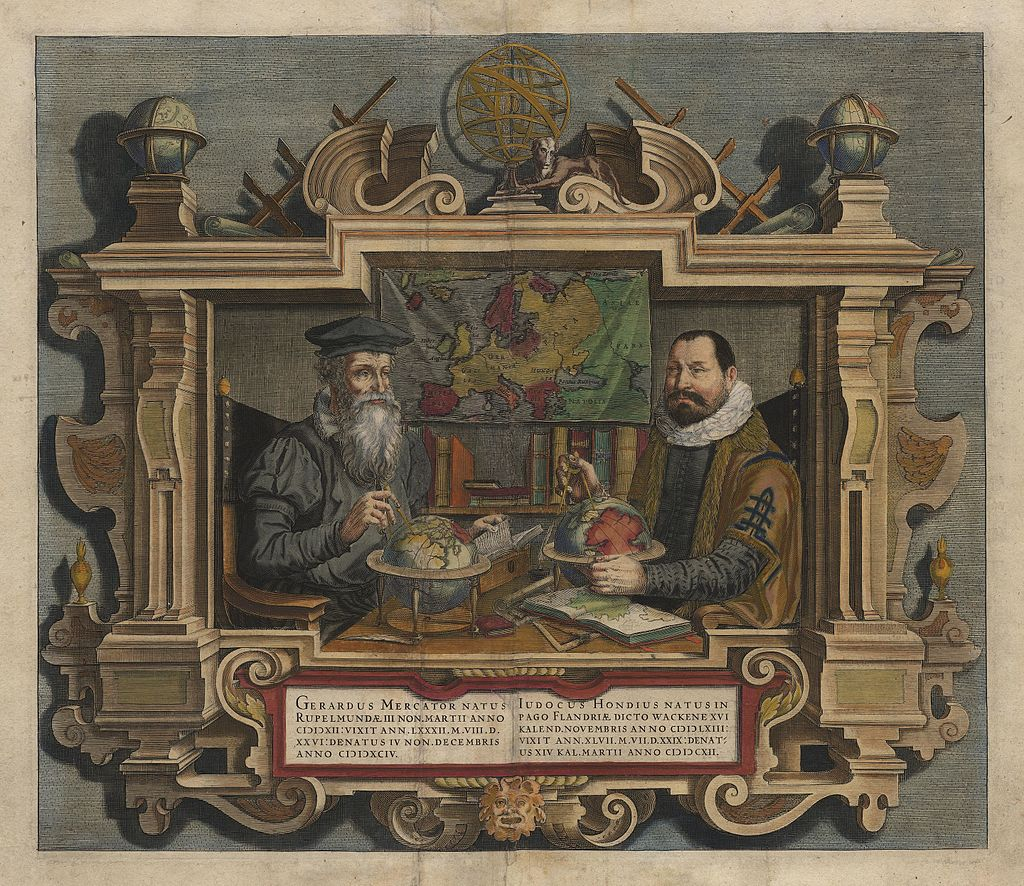
\includegraphics[width=1\linewidth]{../plots/Hondius_Portrait_of_map-makers}
			\caption{Portrait of map-makers, Gerard Mercator and Jodocus Hondius (Jodocus Hondius) source: \url{https://commons.wikimedia.org/wiki/File:Hondius_Portrait_of_map-makers.jpg}}
			\end{figure}
		\end{center}
	\end{column}
	\begin{column}{0.4\linewidth}
		\begin{center}
			\begin{itemize}
				\item<2-> Topography is a description of a landscape
				\item<3-> Topics (from the Greek \textgreek{τόπος}, place) can describe the features of body of text
			\end{itemize}
		\end{center}
	\end{column}
	\end{columns}
\end{frame}

\begin{frame}{Context}

\begin{columns}
	\begin{column}{0.5\linewidth}
		\begin{center}
		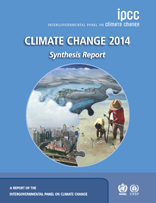
\includegraphics[width=0.6\linewidth]{syrcover.png}
		\end{center}
	\end{column}
	\begin{column}{0.5\linewidth}
	\begin{center}
		\begin{itemize}
			\item To contribute evidence-based policy-making on climate change, the IPCC aims to \textit{comprehensively} assess scientific literature on climate change 
			\item These assessments should be aim to balance legitimacy, credibility and relevance \citep{Cash2001}
		\end{itemize}
	\end{center}
	\end{column}
	\end{columns}

\end{frame}

\begin{frame}{Motivation - Big Literature}

\begin{columns}
	\begin{column}{0.5\linewidth}
		\begin{figure}
		\includegraphics<1>[width=1\linewidth]{../plots/volume_variety_AR0}
		\includegraphics<2>[width=1\linewidth]{../plots/volume_variety_AR1}
		\includegraphics<3>[width=1\linewidth]{../plots/volume_variety_bible_AR1}
		\includegraphics<4>[width=1\linewidth]{../plots/volume_variety_bible_AR2}
		\includegraphics<5>[width=1\linewidth]{../plots/volume_variety_bible_AR3}
		\includegraphics<6>[width=1\linewidth]{../plots/volume_variety_bible_AR4}
		\includegraphics<7>[width=1\linewidth]{../plots/volume_variety_bible_AR5}
		\includegraphics<8->[width=1\linewidth]{../plots/volume_variety_bible_AR6}
		\end{figure}
	\end{column}
	\begin{column}{0.5\linewidth}
		\begin{center}
		\only<1>{\framebox[1.1\width]{A matrix of documents x words } \par}
		\only<2>{\framebox[1.1\width]{AR1: 1,848 documents x 3,528 words } \par}
		\only<3>{\begin{framed}
			The Luther Bible: 1,189 documents (chapters) x 11,973 words
			\end{framed}}
		%\only<3>{\framebox[1.1\width]{The Luther Bible: \par 1,189 documents (chapters) x 11,973 words } \par}
		\only<4>{\framebox[1.1\width]{AR2: 6,941 documents x 15,781 words } \par}
		\only<5>{\framebox[1.1\width]{AR3: 18,728 documents x 27,730 words } \par}
		\only<6>{\framebox[1.1\width]{AR4: 44,000 documents x 45,388 words } \par}
		\only<7>{\framebox[1.1\width]{AR5: 108,277 documents x 75,553 words } \par}
		\only<8->{\framebox[1.1\width]{AR6: 128,357 documents x 86,149 words } \par}
		\end{center}
		\only<9->{		
		\begin{center}
			\begin{itemize}
				\item Comprehensive, credible and relevant assessments become
				more challenging as the literature grows \citep{Minx2017l}
			\end{itemize}
		\begin{remark}[]
			To understand, and to aid, scientific assessments of climate change, we need to machine read the literature
		\end{remark}
		\end{center}
	}
	\end{column}
\end{columns}

\end{frame}



\begin{frame}{Approach - Words, words, words}

\begin{columns}
	\begin{column}{0.5\linewidth}
		\begin{center}
			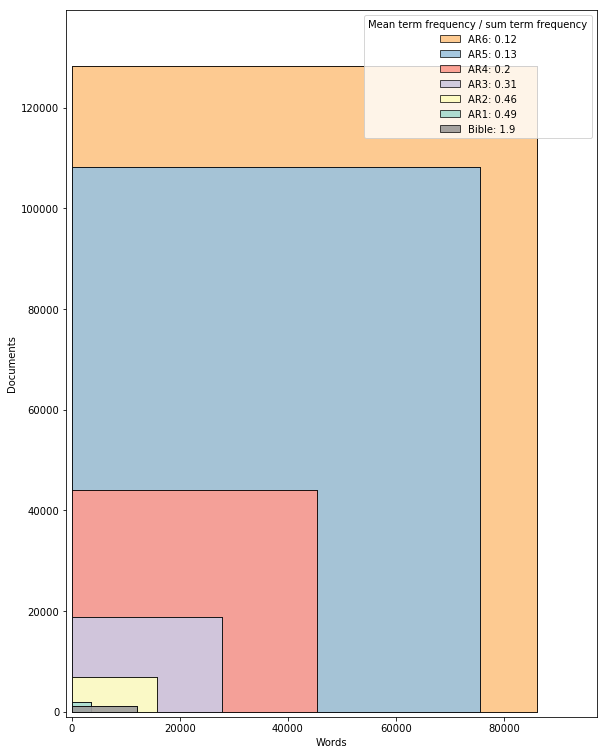
\includegraphics[width=\linewidth]{../plots/volume_variety_bible_AR6}
		\end{center}
	\end{column}
	\begin{column}{0.5\linewidth}
		\textbf{Topic Modelling}
		\begin{center}
			\begin{itemize}
				\item Topic modelling is a way of reducing the dimensionality of a corpus of documents
				\item A large matrix of documents x words is factorised by
				a matrix of topics x words and a matrix of topics x documents
			\citep{Lee1999}
				\item Topics describe the latent structure of the document corpus (What is the matter?)
				
			\end{itemize}
		\end{center}
	\end{column}
\end{columns}

\end{frame}

\begin{frame}{Approach - Words, words, words}

\begin{figure}
	
	\only<1>{\(V_{i\mu} \) is a term frequency-inverse document frequency matrix of \textit{stemmed} terms} 
	\only<2>{\[V_{i\mu} \approx (WH)_{i\mu} = \sum_{a=1}^{r}W_{ia}H_{a\mu} \]} %\(V\) is approximated by the product of \(W\) and \(H\)}
	
	\includegraphics<1>[width=\linewidth]{../plots/VWH_blank.png}
	\includegraphics<2>[width=\linewidth]{../plots/VWH}
	
	\only<1>{\caption{A topic model of 3495 documents on climate change from the year 2000}}
	
	\only<2>{\caption{A topic model of 3495 documents on climate change from the year 2000}}
	
\end{figure}

\end{frame}


%%%%%%%%%%%%%%%%%%%%%%%%

\begin{frame}{Research Questions}
\begin{columns}
	\begin{column}<1->{0.5\linewidth}
		\begin{framed}
			What is the thematic structure of the literature on climate change, and how has this changed over the five assessment periods of the IPCC
		\end{framed}
	\end{column}
	\begin{column}<2->{0.5\linewidth}
		\begin{framed}
			What can this modelled thematic structure tell us about the past and future relationship between the IPCC and scientific literature on climate change? 
		\end{framed}
	\end{column}
\end{columns}

\only<3->{
\textbf{Steps}
\begin{enumerate}
	\item<4-> Download documents from Web of Science (WoS)
	\item<5-> Match documents to reference lists from IPCC reports
	\item<6-> Topic model stemmed document abstracts
\end{enumerate}
}
\end{frame}

%%

\begin{frame}{Data - Query}
\begin{columns}
	\begin{column}{0.65\linewidth}
		\tiny
		(SO=(Climate Alert OR Climate Dynamics OR Climate Policy OR Climatic Change OR Global and Planetary Change OR Global Change Biology OR International Journal of Greenhouse Gas Control OR Mitigation and Adaptation Strategies for Global Change) OR TS=(((CO2 OR "carbon dioxide" OR methane OR CH4 OR "carbon cycle" OR "carbon cycles" OR "carbon cycling" OR "carbon budget*" OR "carbon flux*" OR "carbon mitigation") AND (climat*)) OR (("carbon cycle" OR "carbon cycles" OR "carbon cycling" OR "carbon budget*" OR "carbon flux*" OR "carbon mitigation") AND (atmospher*))) OR TS=("carbon emission*" OR "sequestration of carbon" OR "sequester* carbon" OR "sequestration of CO2" OR "sequester* CO2" OR "carbon tax*" OR "CO2 abatement" OR "CO2 capture" OR "CO2 storage" OR "CO2 sequester*" OR "CO2 sequestration" OR "CO2 sink*" OR "anthropogenic carbon" OR "captur* of carbon dioxide" OR "captur* of CO2" OR "climat* variability" OR "climat* dynamic*" OR "chang* in climat*" OR "climat* proxies" OR "climat* proxy" OR "climat* sensitivity" OR "climat* shift*" OR "coupled ocean-climat*" OR "early climat*" OR "future climat*" OR "past climat*" OR "shift* climat*" OR "shift in climat*") OR TS=("atmospheric carbon dioxide" OR "atmospheric CH4" OR "atmospheric CO2" OR "atmospheric methane" OR "atmospheric N2O" OR "atmospheric nitrous oxide" OR "carbon dioxide emission*" OR "carbon sink*" OR "CH4 emission*" OR "climat* policies" OR "climat* policy" OR "CO2 emission*" OR dendroclimatolog* OR ("emission* of carbon dioxide" NOT nanotube*) OR "emission* of CH4" OR "emission* of CO2" OR "emission* of methane" OR "emission* of N2O" OR "emission* of nitrous oxide" OR "historical climat*" OR IPCC OR "methane emission*" OR "N2O emission*" OR "nitrous oxide emission*") OR TS=("climat* change*" OR "global warming" OR "greenhouse effect" OR "greenhouse gas*" OR "Kyoto Protocol" OR "warming climat*" OR "cap and trade" OR "carbon capture" OR "carbon footprint*" OR "carbon neutral" OR "carbon offset" OR "carbon sequestration" OR "carbon storage" OR "carbon trad*" OR "changing climat*" OR "climat* warming")) NOT PY=2018
		
		\normalsize
		\begin{itemize}
			\item \citep{Haunschild2016}
			\item 309,697 documents
		\end{itemize}
	\end{column}
	\begin{column}{0.35\linewidth}
		\textbf{Caveats}
		\begin{itemize}
			\item Not perfect query
			\item WoS not all peer-reviewed literature
			\item Missing grey literature
			\item Missing relevant literature not directly about climate change
		\end{itemize}
	\end{column}
\end{columns}
\end{frame}

\begin{frame}{Data - IPCC References}
	\textbf{Matching process}
	
	\medskip
	
	For each Reference:
	\begin{itemize}
		\item Check for case-insensitive title matches
		\item Calculate the Jaccard similarity score for two word shingles every database document containing the first word and from the same year. Match if the Jaccard score is above 0.45
	\end{itemize}
\end{frame}


\begin{frame}{Data - IPCC References}
%\begin{columns}
	%\begin{column}{0.5\linewidth}
		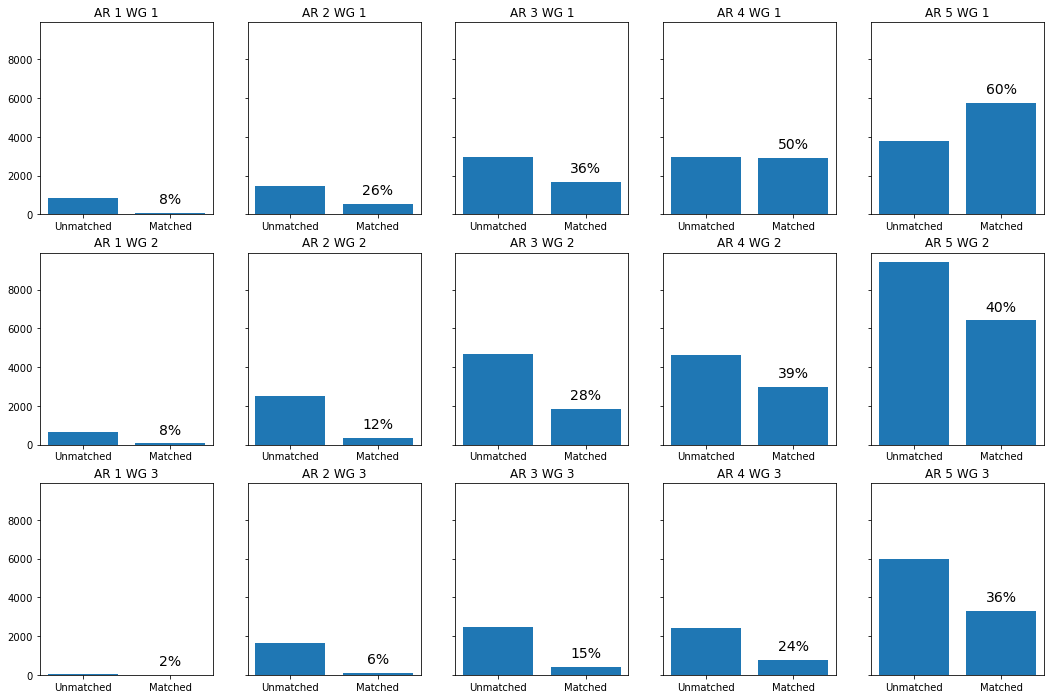
\includegraphics[width=\linewidth]{../plots/ipcc_matches}
	%\end{column}
%\end{columns}
\end{frame}

\begin{frame}{Data - Unmatched IPCC References}
	\tiny
	\begin{tabular}{l l p{4.5cm} p{2.5cm} r}
\toprule
 AR &  WG &                                                                                                                                                                           text &                                                            authors &  year \\
\midrule
 3 &  1 &  The IIASA Database for Mean Monthly   Values of Temperature, Precipitation and Cloudiness on a Global Terrestrial   Grid. IIASA Report RR-91-18, Laxenburg, 63 pp. &  Leemans, R. and W. Cramer &  1991 \\
 2 &  2 &  Rischi connessi con la dinámica glaciale nelle Alpi ItaUane. Geografía Física e Dinámica Quatemaría, 15, 85-99.  &  Dutto, F. and G. Mortara &  1992 \\
 3 &  1 &  Specification   of eddy transfer coefficients in coarse-resolution ocean circulation models.   J. Phys. Oceanogr., 27, 381-402. &  Visbeck, M., J. Marshall, T. Haine and M. Spall &  1997 \\
 3 &  2 &  A koala (Phascolartos   cinereus Goldfuss) population crash during drought and heatwave conditions in   south-western Queensland. Australian Journal of Ecology, 13, 451-461. &  Gordon, G., A.S. Brown, and T. Pulsford &  1988 \\
 4 &  2 &  Climate change and land resources of Russia. &  Isaev, A., V. Stolbovoi, V. Kotlyakov, S. Nilsson and I. McCallum &  2004 \\
 4 &  3 &  Generation technology choices: near and long term. US DOE/EPRI Annual Energy Outlook Conference, Washington D.C., www.eia.doe.gov/oiaf/archive/aeo04/conf/pdf/gehl.pdf  &  Gehl, S &  2004 \\
 4 &  3 &  Climate Change and the European Countryside: Impacts on Land Management and Response Strategies &  Viner, D., M. Sayer, M. Uyarra, and N. Hodgson &  2006 \\
 5 &  2 &  Adaptation to climate change in the context ofsustainable development and equity &  Smit, B. and O. Pilifosova &  2001 \\
 5 &  3 &  Copenhagen City of Cyclists: Bicycle Account 2010. City of Copenha-gen, The Technical and Environmental Administration. Available at: http: / / www. cycling-embassy &  COP &  2010 \\
 5 &  3 &  Uncertainty analysis of the IEA / ORAU CO2 emissions model. The Energy Journal 8, 1 – 29 &  Reilly J M, J A Edmonds, R H Gardner, and A L Brenkert &  1987 \\
\bottomrule
\end{tabular}

\end{frame}

\begin{frame}{Data - Unmatched IPCC References}

37\% of IPCC References could be matched to the database of climate-relevant documents

\medskip

\textbf{Reasons for not matching}
\begin{enumerate}
	\item<2->Reference is not in WoS (not peer-reviewed, in minor journal)
	\item<3->Reference is not directly about climate change
	\item<4->Reference has been incorrectly parsed
\end{enumerate}

\medskip

\only<5->{\textbf{Observations}}
\begin{itemize}
	\item<5-> The size of the literature appears to be \textit{much} bigger than our estimate
	\item<6-> WG3 refers to more literature not directly about climate change, or not in peer-reviewed publications, than WG2, which refers to more than WG1
\end{itemize}

\end{frame}

\begin{frame}{Methodology - Dynamic Topic Modelling}

The topic models above assume that the topics, and the words that make them up, are stable over time. Two approaches to better model dynamic topics:

\begin{itemize}
	\item<2->Dynamic Topic Modelling (DTM) \citep{Blei2006} assume that a constant number of topics exists over all topic models, but allows the words in the topics to evolve from one time period to another
	\item<3->Dynamic Non-negative Matrix Factorisation \citep{Greene2016} has varying numbers of topics in each window and allows for topics to emerge and/or disappear.
\end{itemize}

\onslide<4->{Where the size and variety of the literature we want to model has increased exponentially, we need an approach that allows for the emergence of new topics.}

\end{frame}

%%%%%%%%%%%%%%%%%%%%%%%
%% D-NMF


\begin{frame}[t]{Dynamic NMF}


\only<1->{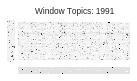
\includegraphics[]{../plots/sustainability/VWH_1991}}
\only<2->{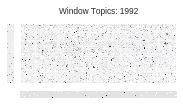
\includegraphics[]{../plots/sustainability/VWH_1992}}

\only<3->{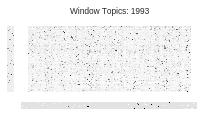
\includegraphics[]{../plots/sustainability/VWH_1993}}

\end{frame}

\begin{frame}[t]{Dynamic NMF}

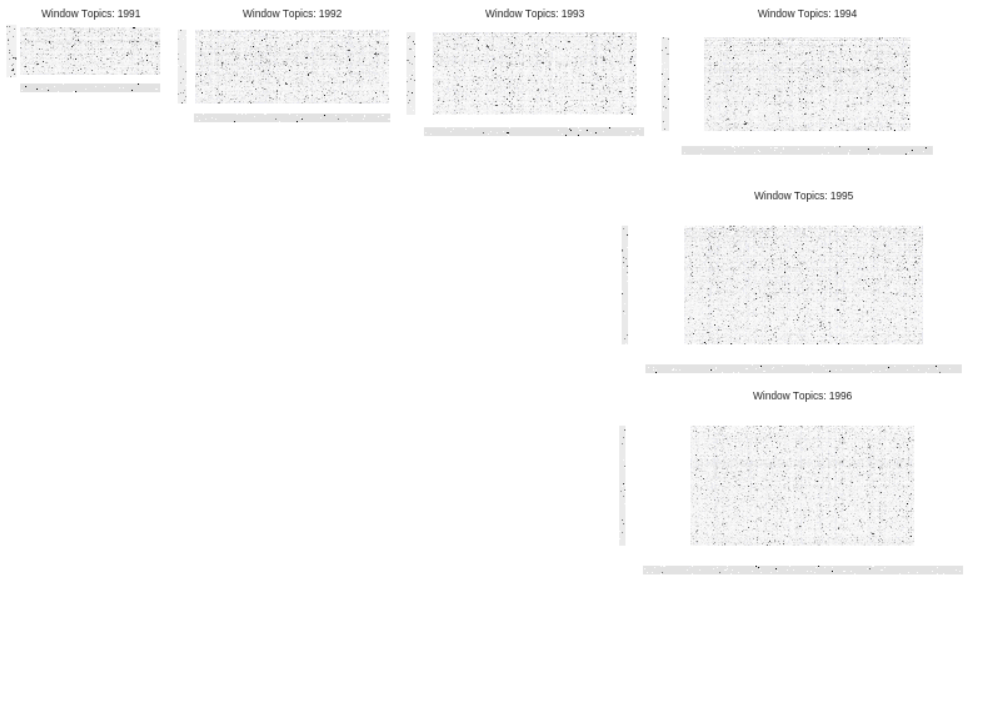
\includegraphics[width=\linewidth]{../plots/sustainability/conceptual_windows_only}

\end{frame}

\begin{frame}[t]{Dynamic NMF}

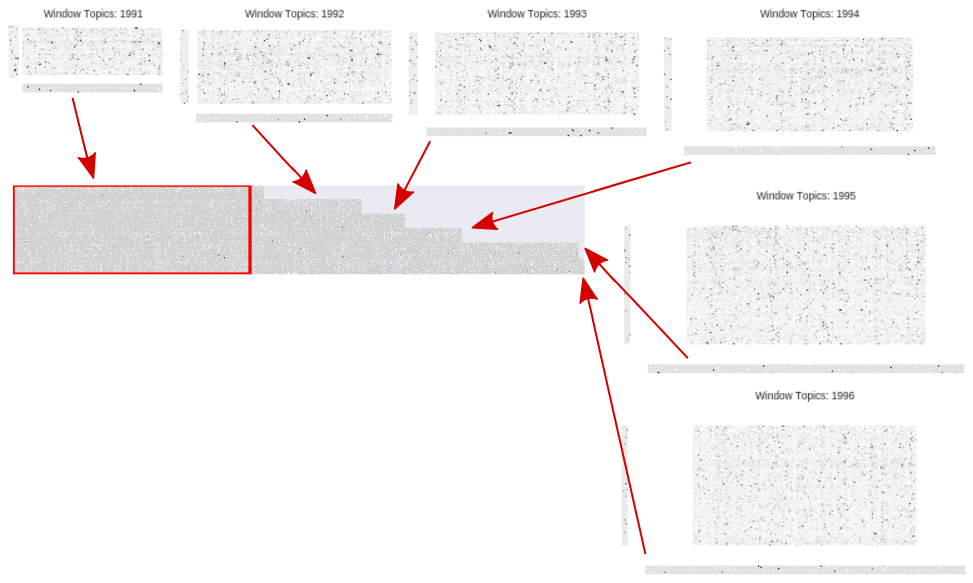
\includegraphics[width=\linewidth]{../plots/sustainability/conceptual_annotated_1}

\end{frame}

\begin{frame}[t]{Dynamic NMF}

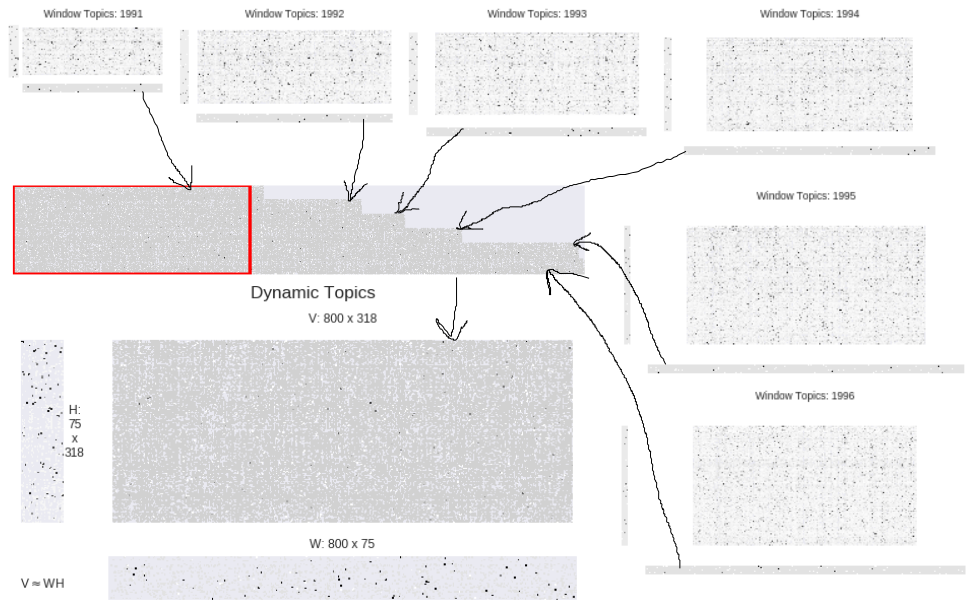
\includegraphics[width=\linewidth]{../plots/sustainability/conceptual_annotated_2}

\end{frame}


\begin{frame}{Dynamic NMF - application to climate change}

\onslide<1->{
\begin{itemize}
	\item Choosing the number of window topics is non-trivial. Data-driven approaches are limited (see below), and human selection is time consuming.
	\item To facilitate the description of trends over the assessment periods of the IPCC, and to minimize the number of modelling decisions, I consider each IPCC assessment period as a time window.
\end{itemize}}

\begin{columns}
	\onslide<2->{
	\begin{column}{0.5\linewidth}

			\begin{itemize}
				\item Starting from a logarithmic relationship between the number of documents and the ideal topic number, I compare 5 runs with varying numbers of topics for each window
		\end{itemize}
	\end{column}
	\begin{column}{0.5\linewidth}
		\begin{figure}
			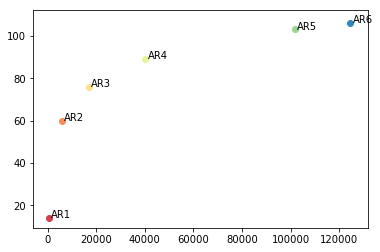
\includegraphics[width=\linewidth]{../plots/n_topics}	
		\end{figure}
	\end{column}
}
\end{columns}

\end{frame}





\begin{frame}[t]{Dynamic NMF - number of topics}

\begin{columns}
	\begin{column}{0.5\linewidth}
		\textbf{Human topic number criteria}
		\begin{itemize}
			\item Intelligibility
		\end{itemize}
		\textbf{Data-driven topic number criteria}
		\begin{itemize}
			\item Reconstruction accuracy
			\item Predictive capacity
		\end{itemize}
		\onslide<2->{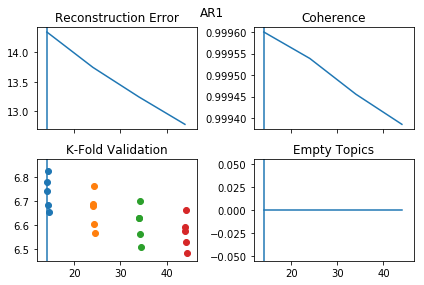
\includegraphics[width=0.8\linewidth]{../plots/topic_validations_AR1}}
	\end{column}
	\begin{column}<2->{0.5\linewidth}
		
\begin{figure}
	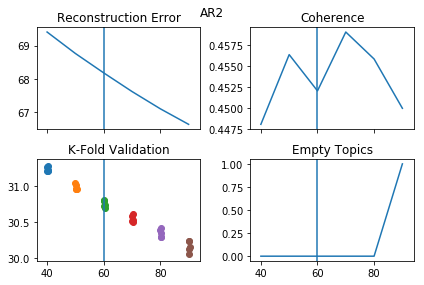
\includegraphics[width=0.8\linewidth]{../plots/topic_validations_AR2}
	
	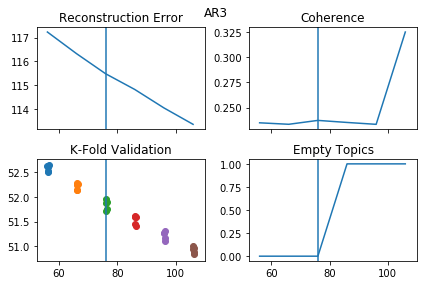
\includegraphics[width=0.8\linewidth]{../plots/topic_validations_AR3}
\end{figure}
	\end{column}
\end{columns}


\end{frame}


%%%%%%%%%%%%%%%%%%%%%%%%%%%%%%%%%%%
% results

\begin{frame}{Results}

\begin{columns}
	\begin{column}{0.5\linewidth}
		\begin{center}	
			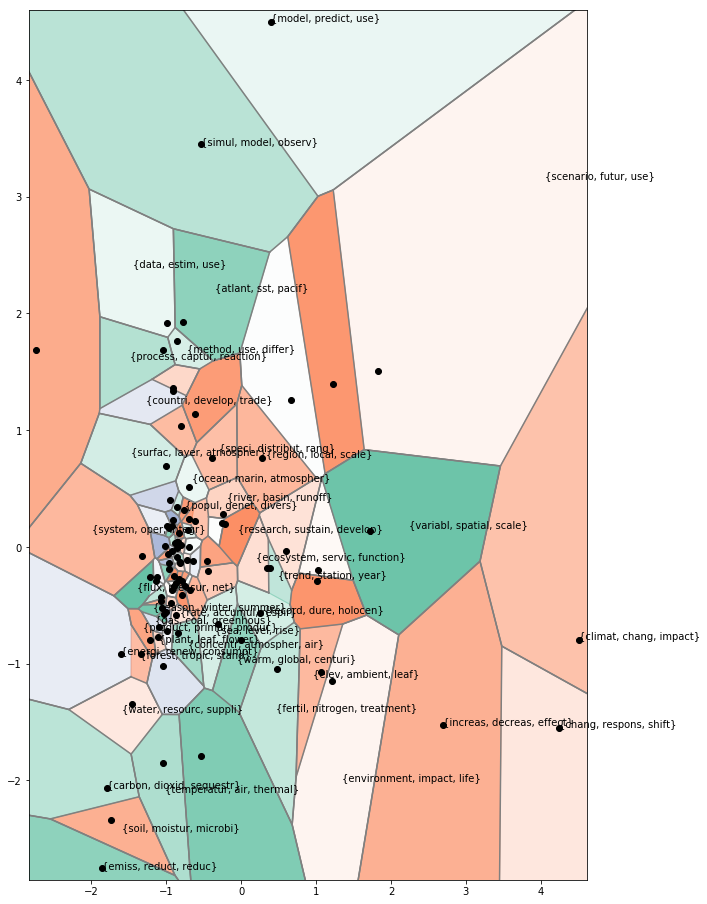
\includegraphics[width=\linewidth]{../plots/pca_map_portrait}
		\end{center}
	\end{column}
	\begin{column}{0.5\linewidth}
		\textbf{Outline}	
		\begin{center}
			\begin{itemize}
				\item<2-> Topography
				\item<3-> Structure
				\item<4-> Development
				\item<5-> Representation in past IPCC reports
				\item<6-> AR6 outlook
			\end{itemize}
		\end{center}
	\end{column}
\end{columns}

\end{frame}


%\begin{frame}{Preliminary results - explanation}
%
%\begin{columns}
%	\begin{column}{0.5\linewidth}
%		\begin{center}
%			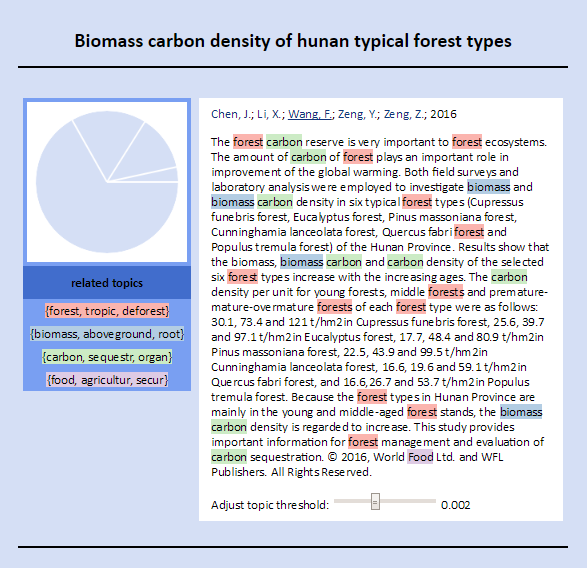
\includegraphics[width=\linewidth]{../plots/biomass_eg.png}
%		\end{center}
%	\end{column}
%	\begin{column}{0.5\linewidth}
%		\begin{center}
%			\begin{itemize}
%				\item Documents are mixtures of topics, based on the words which occur in them
%			\end{itemize}
%		\end{center}
%	\end{column}
%\end{columns}
%
%\end{frame}

%\begin{frame}{Preliminary results - Map}
%
%\begin{figure}
%			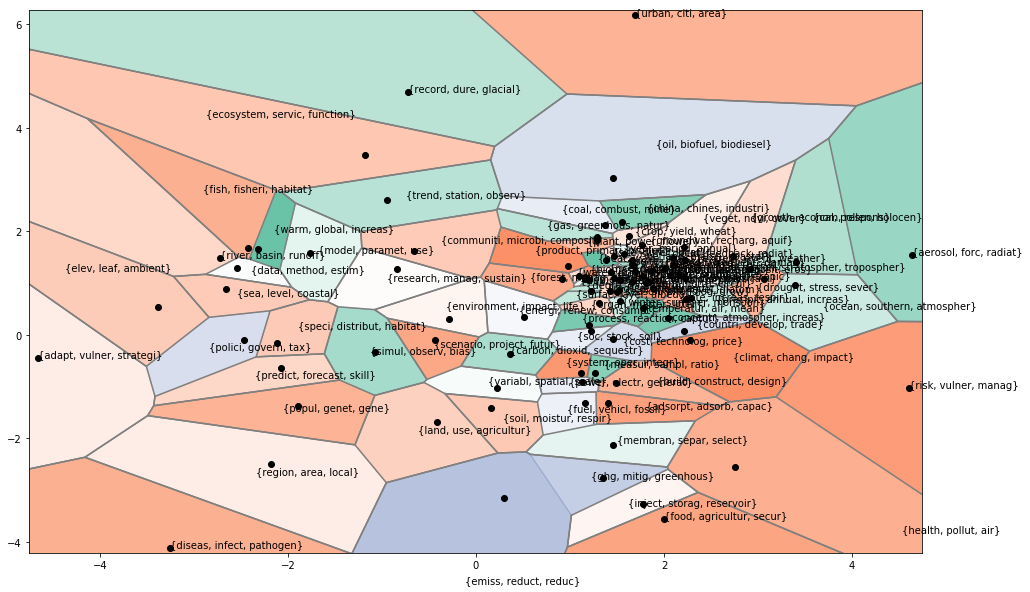
\includegraphics[width=\linewidth]{../plots/pca_map.png}
%			\caption{Topic Map, with topics placed according to Principal Component Analysis of topic-term matrix}
%\end{figure}
%
%\end{frame}


\begin{frame}{Results - structure}

\begin{columns}
	\begin{column}{0.65\linewidth}
		\begin{center}	
			\vspace*{-0.1\linewidth}
			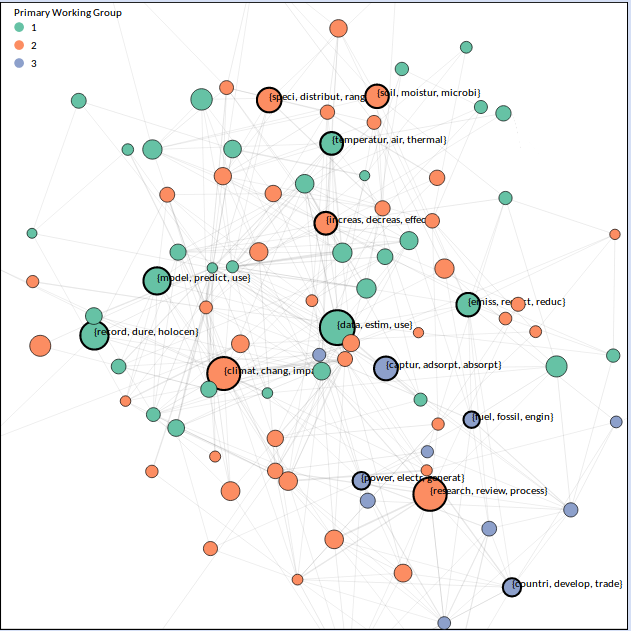
\includegraphics[width=\linewidth]{../plots/network_wg_654}
		\end{center}
	\end{column}
	\begin{column}{0.35\linewidth}
	%	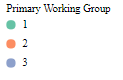
\includegraphics[width=0.4\linewidth]{../plots/network_wg_key}
		\begin{center}
			\begin{itemize}
				\item<1-> Topics describe comprehensible themes in climate change research
				\item<2-> Matching topics to the IPCC working group from which the majority of the topics are referenced in, a structure is generated based on topic-document correlations
			\end{itemize}
		\end{center}
	\end{column}
\end{columns}

\end{frame}


\begin{frame}{Results - Inter-working Group topics - WG 1 and 2}
	
	\begin{table}
		
		
		\begin{tabular}{p{1.4cm} p{1cm} l r r r}
\toprule
 IPCC Coverage &  Primary WG &               Topic Title &  WG 1 &  WG 2 &  WG 3 \\
\midrule
         0.16\% &           1 &  \{rainfal, monsoon, rain\} & 0.50\% & 0.50\% & 0.00\% \\
         0.10\% &           2 &      \{veget, ndvi, cover\} & 0.41\% & 0.59\% & 0.00\% \\
         0.16\% &           1 &     \{snow, cover, winter\} & 0.59\% & 0.41\% & 0.00\% \\
         0.17\% &           2 &    \{region, local, scale\} & 0.41\% & 0.59\% & 0.00\% \\
         0.16\% &           1 &  \{coastal, mangrov, rise\} & 0.57\% & 0.42\% & 0.01\% \\
\bottomrule
\end{tabular}

		
	\end{table}
	
\end{frame}

\begin{frame}{Results - Inter-working Group topics - WG 1 and 3}

\begin{table}
	
	
	\begin{tabular}{p{1.4cm} p{1cm} l r r r}
\toprule
 IPCC Coverage &  Primary WG &                   Topic Title &  WG 1 &  WG 2 &  WG 3 \\
\midrule
         0.09\% &           3 &        \{gas, coal, greenhous\} & 0.30\% & 0.15\% & 0.56\% \\
         0.10\% &           3 &     \{transport, vehicl, road\} & 0.24\% & 0.12\% & 0.64\% \\
         0.13\% &           1 &        \{emiss, reduct, reduc\} & 0.45\% & 0.21\% & 0.34\% \\
         0.09\% &           1 &  \{methan, oxid, methanotroph\} & 0.63\% & 0.16\% & 0.20\% \\
         0.13\% &           3 &         \{ghg, greenhous, gas\} & 0.15\% & 0.09\% & 0.75\% \\
\bottomrule
\end{tabular}

	
\end{table}

\end{frame}

%%%%%%%

\begin{frame}{Results - Inter-working Group topics - WG 2 and 3}

\begin{table}


\begin{tabular}{p{1.4cm} p{1cm} l r r r}
\toprule
 IPCC Coverage &  Primary WG &                  Topic Title &  WG 1 &  WG 2 &  WG 3 \\
\midrule
         0.11\% &           2 &  \{sustain, develop, resourc\} & 0.04\% & 0.51\% & 0.46\% \\
         0.08\% &           3 &   \{build, construct, design\} & 0.03\% & 0.38\% & 0.59\% \\
         0.11\% &           2 &  \{environment, impact, life\} & 0.06\% & 0.58\% & 0.36\% \\
         0.19\% &           3 &        \{polici, tax, govern\} & 0.02\% & 0.32\% & 0.66\% \\
         0.16\% &           2 &          \{urban, citi, plan\} & 0.07\% & 0.55\% & 0.38\% \\
\bottomrule
\end{tabular}


\end{table}

\end{frame}

%%%%%%%%
%% RESULTS - DEVELOPMENT
%\begin{frame}{Results - Development}
%\only<1->{
%\begin{figure}
%	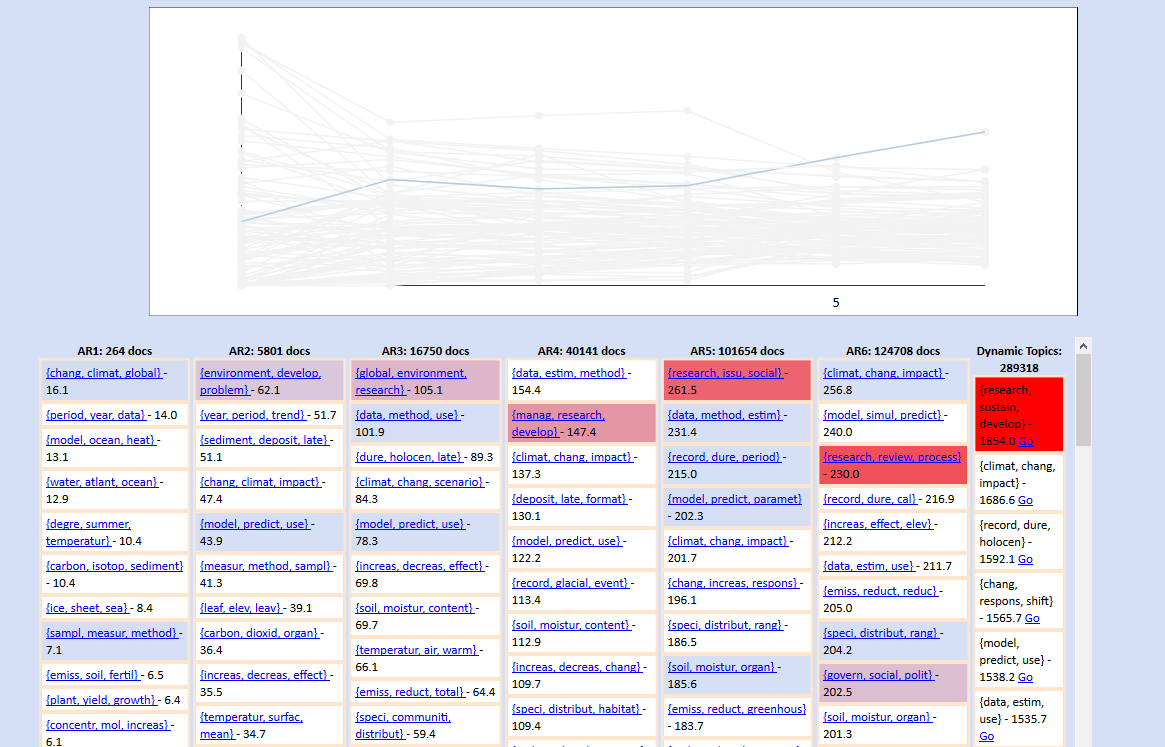
\includegraphics[width=0.8\linewidth]{../plots/development/662_sus}	
%\end{figure}
%}
%\only<1->{
%	\centering
%	\textbf{Message}
%}
%\end{frame}

\begin{frame}{Results - Development}
\only<1->{
	\begin{figure}
		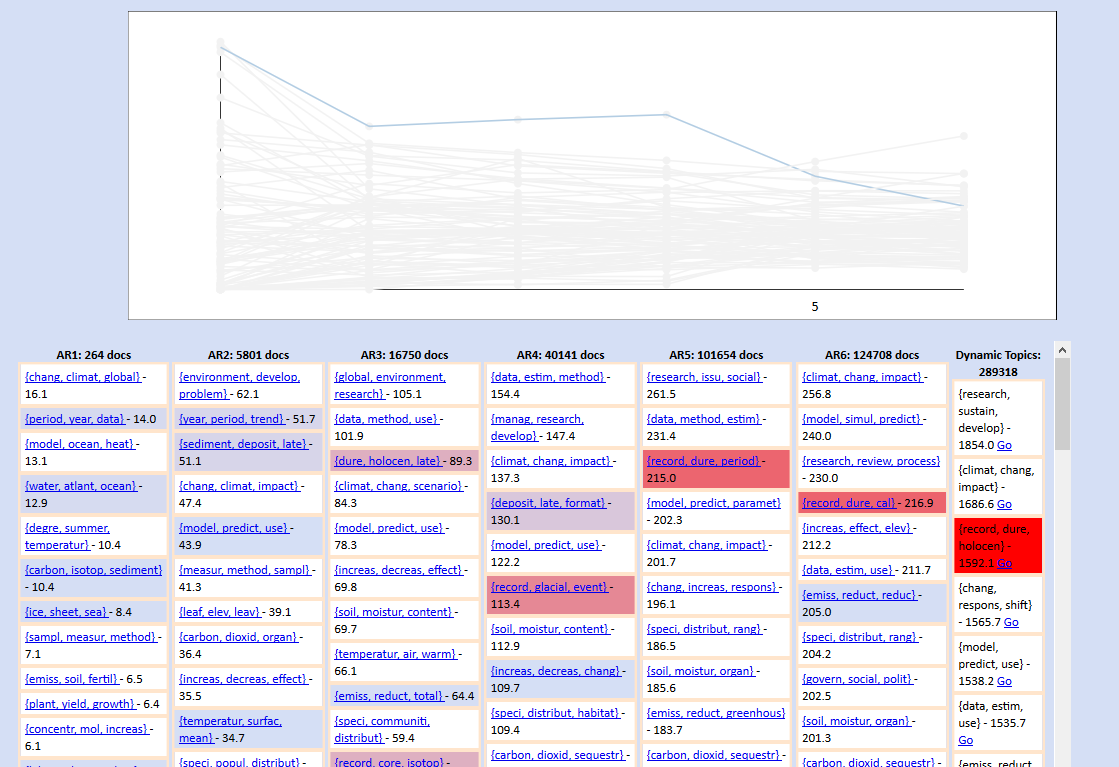
\includegraphics[width=0.8\linewidth]{../plots/development/662_holocene}	
	\end{figure}
}
\only<1->{
	\centering
	\textbf{Basic climate science topics are not as prominent as they were previously}
}
\end{frame}

\begin{frame}{Results - Development}
\only<1->{
	\begin{figure}
		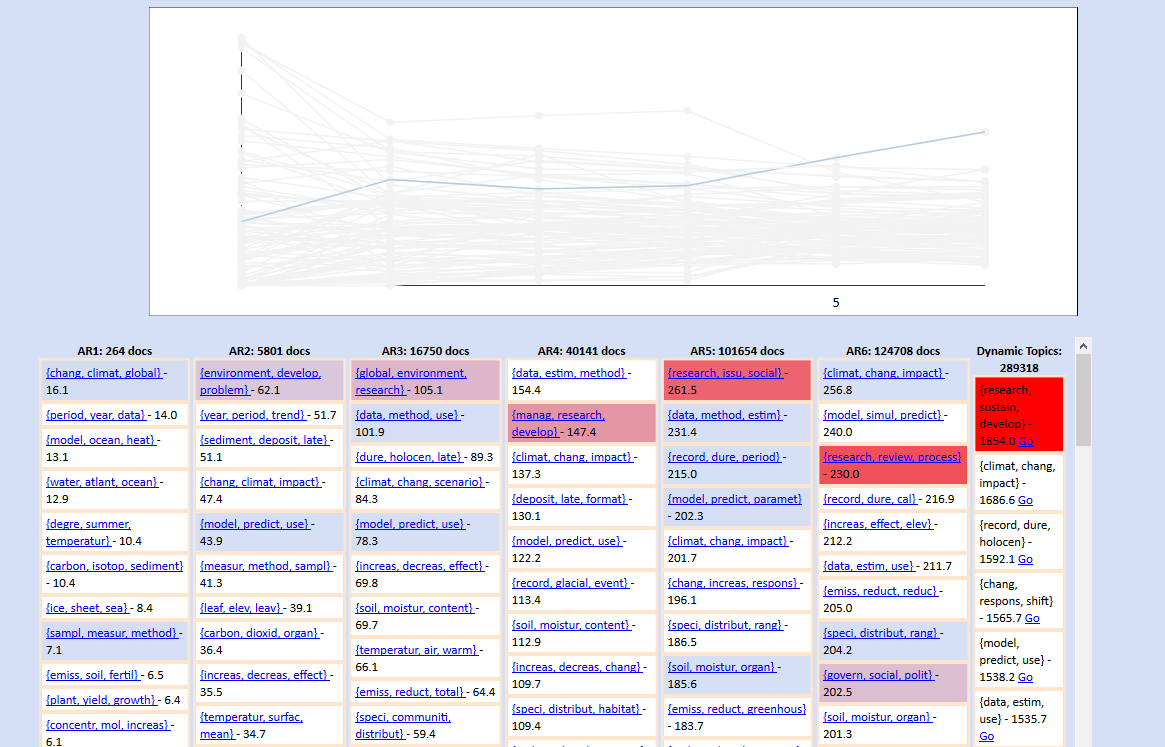
\includegraphics[width=0.8\linewidth]{../plots/development/662_sus}	
	\end{figure}
}
\only<1->{
	\centering
	\textbf{Sustainable development, and research agendas are more prominent}
}
\end{frame}


\begin{frame}
	\begin{figure}
		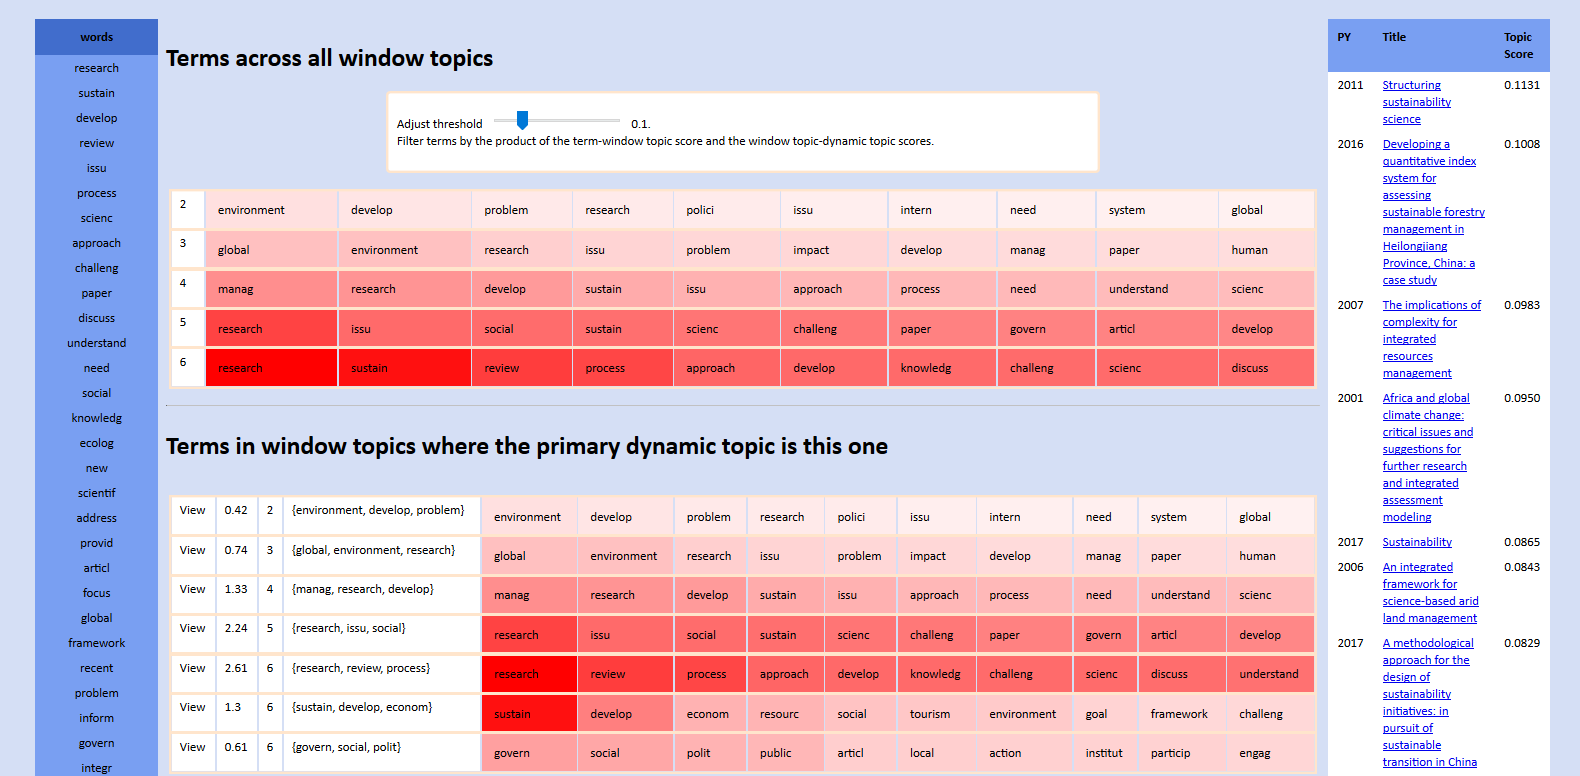
\includegraphics[width=\linewidth]{../plots/sus_overview}
	\end{figure}
\end{frame}

\begin{frame}{Results - Development}
\only<1->{
	\begin{figure}
		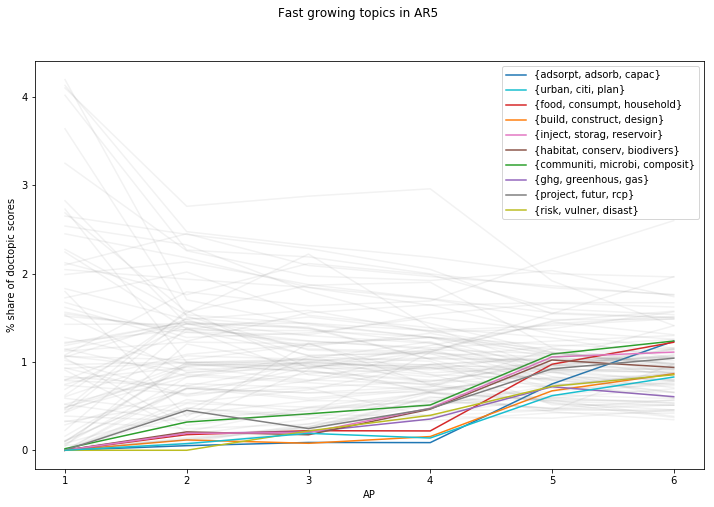
\includegraphics[width=0.8\linewidth]{../plots/ar5_growth_662}	
	\end{figure}
}
\only<1->{
	\centering
	\textbf{Fast growing topics in AR5 were on urban systems, negative emissions, buildings, consumption, biodiversity and risks}
}
\end{frame}

\begin{frame}{Results - Development}
\only<1->{
\begin{figure}
	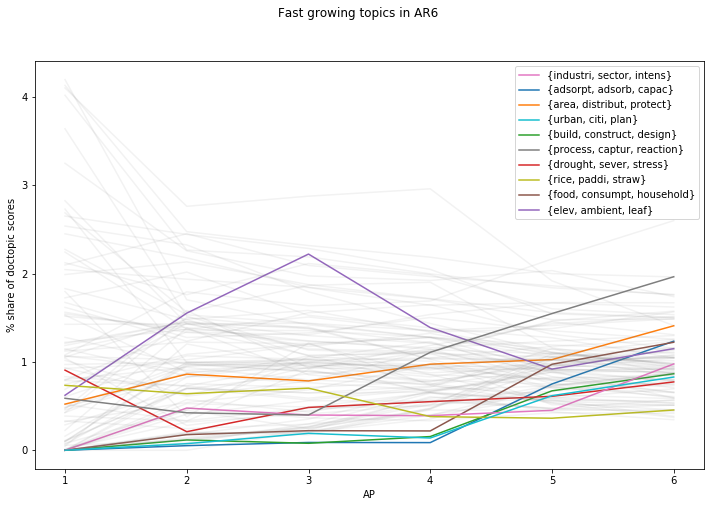
\includegraphics[width=0.8\linewidth]{../plots/ar6_growth_662}	
\end{figure}
}
\only<1->{
	\centering
	\textbf{Negative emissions topics continue to grow,}
}
\end{frame}


%%%%%%%%%


\begin{frame}{Results - topic representation in IPCC reports}

\begin{itemize}
	\item<1-> How can we get a sense of which topics are better covered in IPCC reports?
	\item<2-> We get a measure of proportionality between two distributions by dividing the each topics share in the IPCC sample by its share in the whole corpus
	\item<3-> This and other measures come from literature on the proportionality of electoral systems \citep[e.g][]{Karpov2008}
\end{itemize}



\medskip



%\begin{itemize}
%	\item Each document \(d\) either matches or does not match an IPCC reference
%	\item For each topic \(h\), we can sum the scores for each category of document
%	\item The ``IPCC proportion'' of each topic is the proportion of the sum of the document score accounted for by documents which match IPCC references.
%\end{itemize}

\end{frame}

\begin{frame}{Results - topic representation in IPCC reports}

\begin{columns}
	\begin{column}{0.7\linewidth}
		\begin{center}
			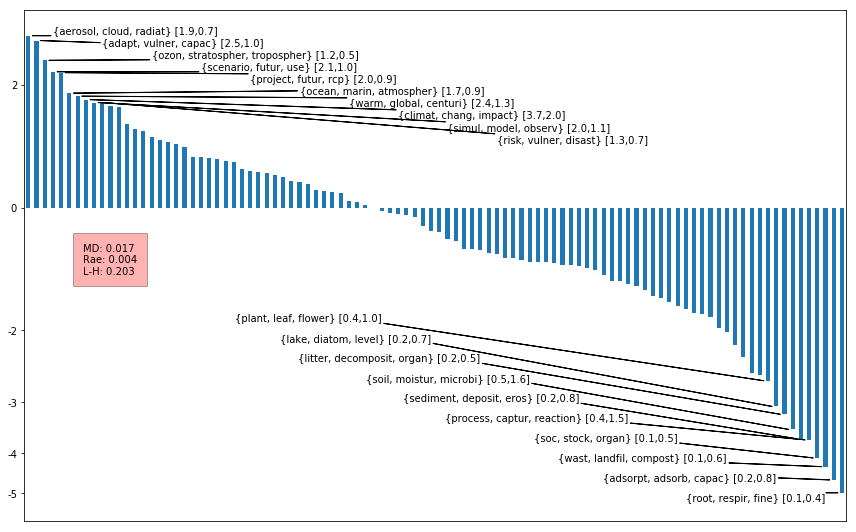
\includegraphics[width=\linewidth]{../plots/ipcc_representation/ipcc_rep_662_all.png}
		\end{center}
	\end{column}
	\begin{column}{0.3\linewidth}
		\begin{center}
			\begin{itemize}
				\item The physical science aspects of climate change, as well topics on impacts, adaptation and scenarios are well covered by the IPCC
				\item Topics on specific technological solutions (particularly NETs), as well as soils and plants are less well represented
			\end{itemize}
		\end{center}
	\end{column}
\end{columns}

\end{frame}



\begin{frame}{Results - topic representation in IPCC reports}

	\begin{figure}
			\includegraphics[width=0.8\linewidth]{../plots/ipcc_representation/ipcc_rep_662_ARs}
	\end{figure}

\end{frame}

\begin{frame}{Results - topic representation in IPCC reports}

\begin{columns}
	\begin{column}{0.7\linewidth}
				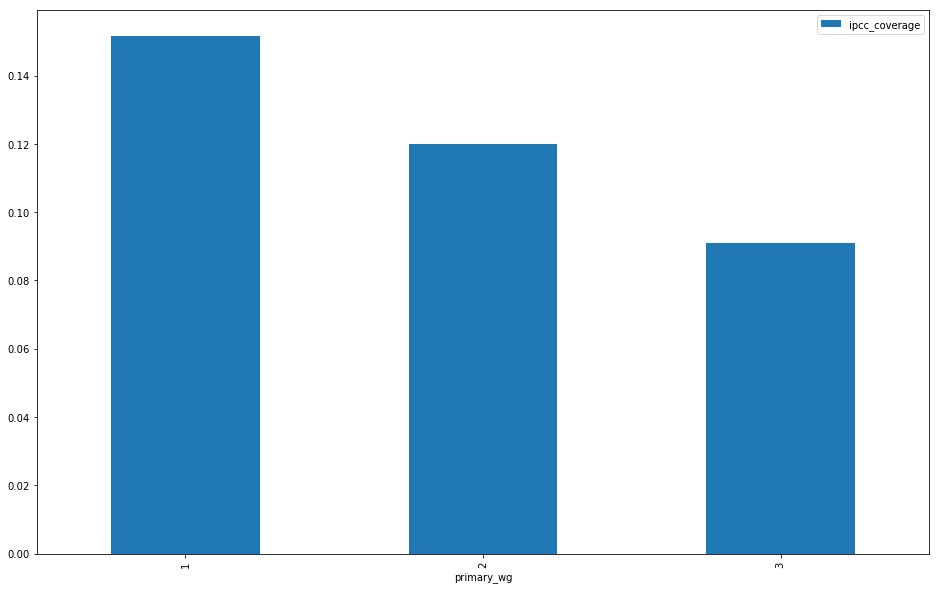
\includegraphics[width=\linewidth]{../plots/ipcc_coverage_by_wg_654.png}
	\end{column}
	\begin{column}{0.3\linewidth}
		\begin{itemize}
			\item On average, topics that are primarily referenced by working group I report have a higher proportion of constituent documents matching IPCC references
		\end{itemize}
	\end{column}
\end{columns}

	
	
\end{frame}





\begin{frame}{Results - AR6 outlook}

\begin{itemize}
	\item<1-> Outlines for the sixth assessment report have already been published
	\item<2-> The words in each chapter were matched to the Topic-Term matrix generated by the model to calculate a simplified topic score for each chapter
	\item<3-> These scores were summed and were compared to the corpus in general in the same way as with past reports
\end{itemize}



\end{frame}


\begin{frame}{Results - topic representation in IPCC reports}

\begin{columns}
	\begin{column}{0.7\linewidth}
		\begin{center}
			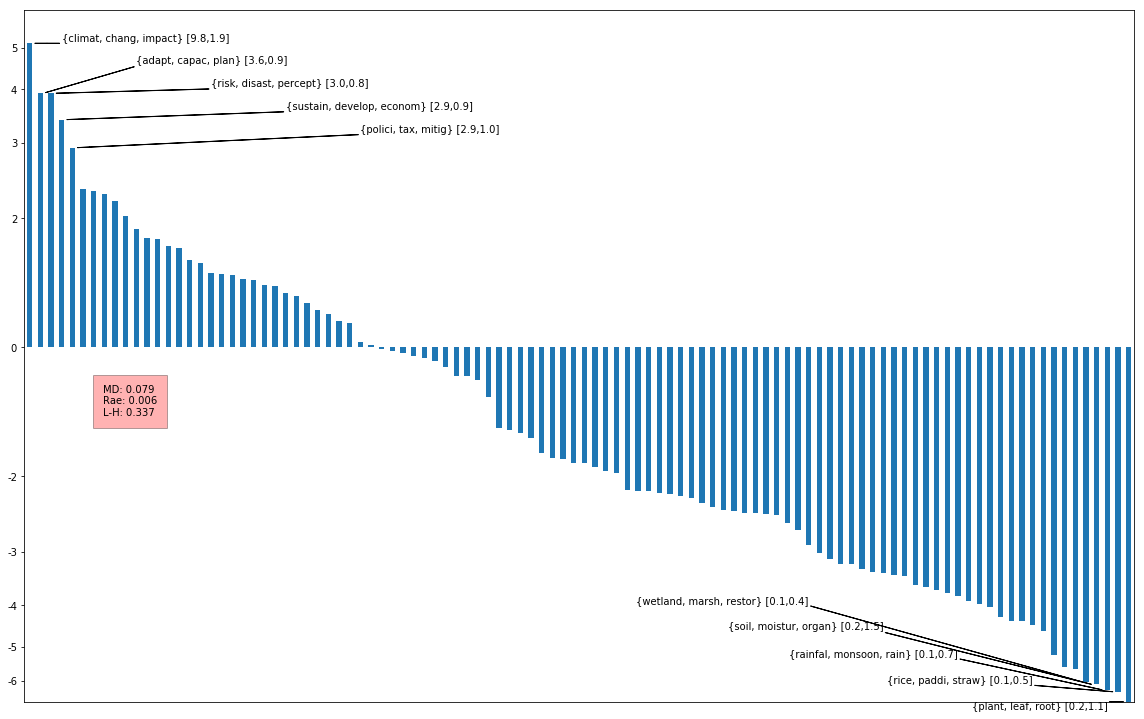
\includegraphics[width=\linewidth]{../plots/ipcc_representation/ipcc_rep_662_AR6.png}
		\end{center}
	\end{column}
	\begin{column}{0.3\linewidth}
		\begin{center}
			\begin{itemize}
				\item The physical science aspects of climate change, as well topics on impacts, adaptation and scenarios are well covered by the IPCC
				\item Topics on specific technological solutions (particularly NETs), as well as soils and plants are less well represented
			\end{itemize}
		\end{center}
	\end{column}
\end{columns}

\end{frame}

\begin{frame}{Robustness}

Most work focuses on the measuring the sensitivity of the reconstruction error to different framings and parameters of the model. What we are more interested in is checking if the key messages are sound.

\begin{columns}<2->
	\begin{column}<3->{0.33\linewidth}
		\begin{figure}
			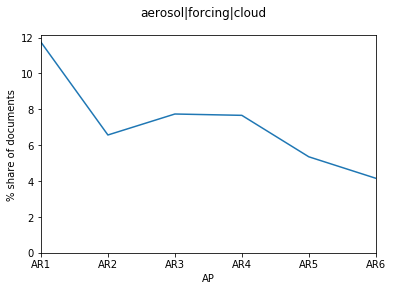
\includegraphics[width=\linewidth]{../plots/aero_share}
		\end{figure}
	\end{column}

	\begin{column}<4->{0.33\linewidth}
		\begin{figure}
			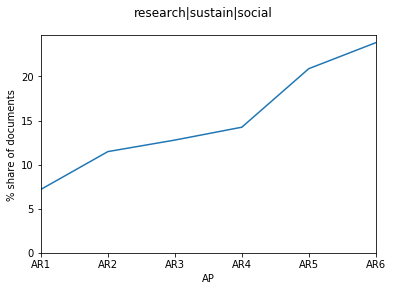
\includegraphics[width=\linewidth]{../plots/sus_share}
		\end{figure}
	\end{column}

\end{columns}
\begin{columns}

	\begin{column}<5->{0.33\linewidth}
		\begin{figure}
			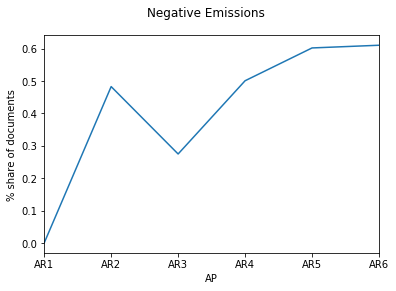
\includegraphics[width=\linewidth]{../plots/negative_emissions_share}
		\end{figure}
	\end{column}

	\begin{column}<6->{0.33\linewidth}
	\begin{figure}
		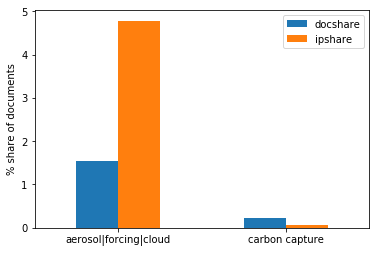
\includegraphics[width=\linewidth]{../plots/ipcc_rep_simple}
	\end{figure}
	\end{column}
\end{columns}

\end{frame}


%\begin{frame}{Next steps}
%	\begin{itemize}
%		\item Adjusting second stage of model to give more weight to topics with many documents (to better capture emergence)
%		\item Further analysis of new model
%		\item (Manual) comparison of (AR6) topics with AR6 outline
%	\end{itemize}
%\end{frame}

\begin{frame}{Conclusions}


\begin{itemize}
	\item<1-> Endogenously discovered topics map and make substantive sense of an unmanageable dataset of climate-relevant literature
	\item<2-> Topic modelling discovers over-arching topics such as that on sustainability and research priorities, as well as specific, fast growing topics such those on negative emissions
	\item<3-> Some quantitative evidence is found to support policy makers' dissatisfaction with a lack of `solution orientation' in IPCC reports \citep{Kowarsch2017} 
\end{itemize}

\end{frame}

\begin{frame}{Discussion}


\begin{itemize}
	\item<1-> A perfectly representative relationship between the literature and IPCC reports is not necessarily desirable
	\item<2-> The IPCC are best placed to decide which aspects of the literature to emphasise
	\item<3-> A topography of the literature helps to address issues of emphasis from a point of understanding, and to make decisions clear and transparent
	\item<4-> More generally, maps like this present exciting opportunities to aid the process of literature selection, and to understand the science policy process
\end{itemize}

\end{frame}


%\begin{frame}{Extra results - Journals}
%
%\begin{columns}
%	\begin{column}{0.55\linewidth}
%		\begin{center}
%			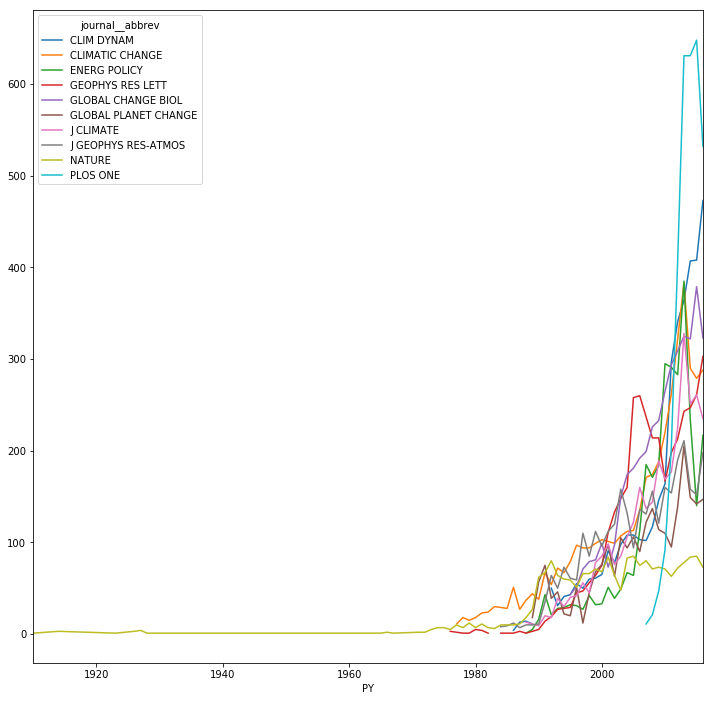
\includegraphics[width=\linewidth]{../plots/journals/journal_papers.png}
%		\end{center}
%	\end{column}
%	\begin{column}{0.45\linewidth}
%		\begin{center}
%			\begin{itemize}
%				\item Nature has been publishing about climate change for a long time
%				\item Plos One has very recently overtaken all other journals
%				\item The number of journals has risen very steeply
%			\end{itemize}
%		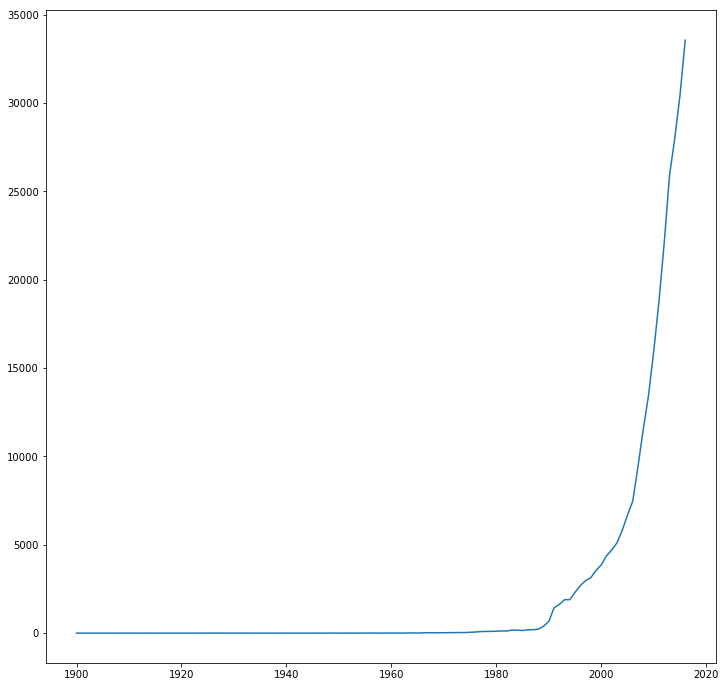
\includegraphics[width=0.9\linewidth]{../plots/journals/n_journals.png}
%		\end{center}
%	\end{column}
%\end{columns}
%
%\end{frame}

%\begin{frame}{Extra results - Journals}

%\begin{columns}
%	\begin{column}{0.55\linewidth}
%		\begin{center}
%			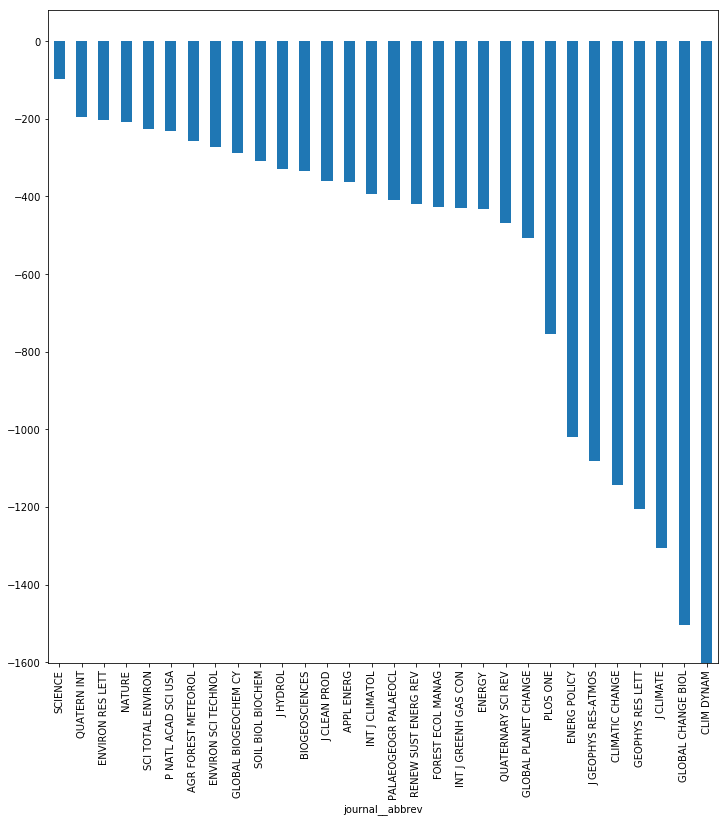
\includegraphics[width=\linewidth]{../plots/journals/journal_entropy_386.png}
%		\end{center}
%	\end{column}
%	\begin{column}{0.45\linewidth}
%		\begin{center}
%			\begin{itemize}
%				\item Journal Entropy describes the distribution of topics in a journal \citep{Hall2008a}
%				\item High values mean the journal deals with a wider range of topics
%			\end{itemize}
%			\[  H(z\rvert c,y) = -\sum_{i=1}^{K} \hat{p}(z_i \rvert c,y) \; log \; \hat{p}(z_i \rvert c, y) \]
%		\end{center}
%	\end{column}
%\end{columns}
%
%\end{frame}

%\begin{frame}{Extra results - Journals}
%
%	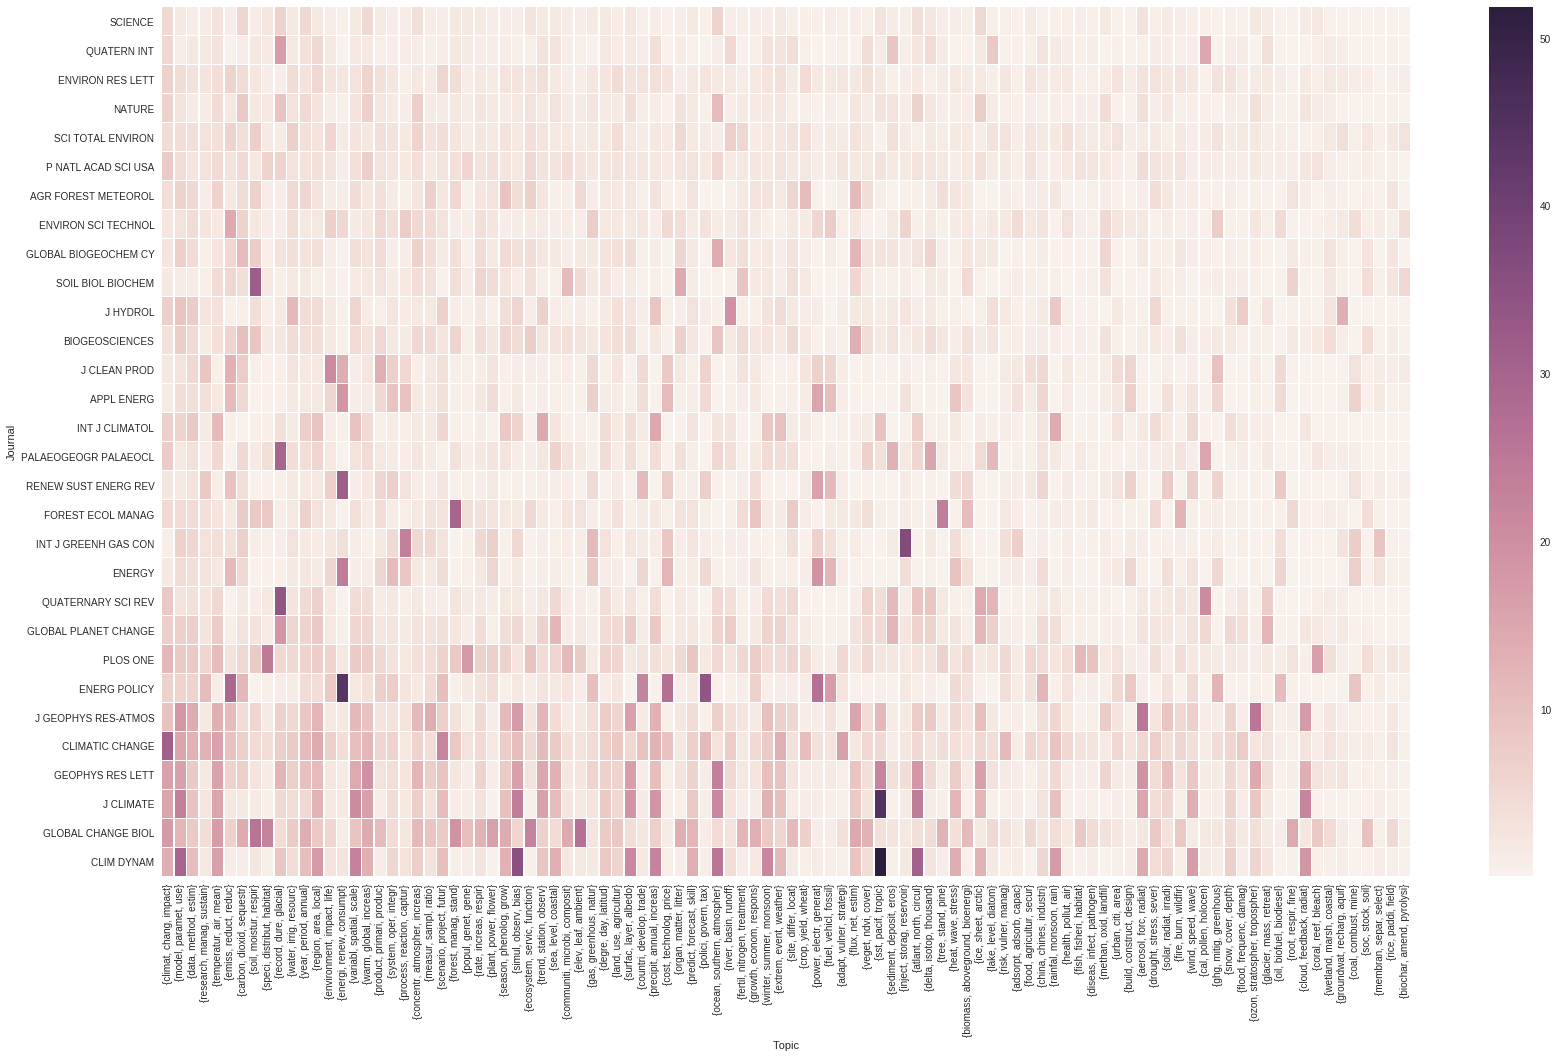
\includegraphics[width=\linewidth]{../plots/journals/journal_topics_386.png}
%
%\end{frame}


%\begin{frame}{Outlook}
%
%\begin{figure}
%
%\tiny
%
%\begin{ganttchart}[
%	y unit title=0.3cm,
%	y unit chart=0.5cm,
%	x unit= 0.2cm,
%	vgrid,hgrid,
%	vgrid={{dotted,dotted,black}},
%	title height=1,
%	%     title/.style={fill=none},
%	title label font=\bfseries\scriptsize,
%	%bar/.style={fill=blue},
%	bar height=0.7,
%	bar label font=\tiny,
%	%   progress label text={},
%	group right shift=0,
%	group top shift=0.7,
%	group height=.3,
%	group peaks width={0.2},
%	inline]{1}{42}
%	\gantttitle{2017}{9}
%	\gantttitle{2018}{12}
%	\gantttitle{2019}{12}
%	\gantttitle{2020}{9} \\
%	\gantttitlelist{2,...,4}{3} \gantttitlelist{1,...,4}{3} \gantttitlelist{1,...,4}{3} \gantttitlelist{1,...,3}{3} \\
%	\gantttitlelist{4,...,12}{1} \gantttitlelist{1,...,12}{1}
%	%\gantttitlelist{J,F,M,A,M,J,J,A,S,O,N,D}{1}
%	\gantttitlelist{1,...,12}{1} \gantttitlelist{1,...,9}{1}\\
%	
%	% HERTIE
%	\ganttgroup[inline=false]{Hertie Courses}{6}{42} \\
%	
%	\ganttbar[inline=false, bar/.append style={fill=rd}]{Research Design}{6}{15} \\
%	\ganttbar[inline=false, bar/.append style={fill=methods}]{Methods}{6}{15} \\
%	\ganttbar[inline=false, bar/.append style={fill=skills}]{Skills}{6}{15} \\
%	\ganttbar[inline=false, bar/.append style={fill=rc}]{Research Colloquium}{19}{42} \\
%	
%	% HERTIE
%	\ganttgroup[inline=false]{Thesis Research}{1}{42} \\
%	\ganttbar[inline=false, bar/.append style={fill=research}]{Knowledge Map}{1}{5} \\
%	\ganttbar[inline=false, bar/.append style={fill=research}]{Pyramid}{6}{15} \\
%	
%	
%	\ganttbar[inline=false, bar/.append style={fill=research}]{Knowledge Accumulation}{16}{27} \\
%	
%	\ganttbar[inline=false, bar/.append style={fill=research}]{Evidence in Policy}{19}{27} \\
%	
%	\ganttbar[inline=false, bar/.append style={fill=research}]{Envelope}{28}{33} \\
%	
%	\ganttbar[inline=false, bar/.append style={fill=research}]{Revisions/Contingency}{34}{42} \\
%	
%	%\ganttlinkedbar[inline=false]{Task 2}{3}{7} \ganttnewline
%	%\ganttmilestone[inline=false]{Milestone}{7} \ganttnewline
%	
%	
%	
%\end{ganttchart} 
%
%\end{figure}
%
%\end{frame}

\begin{frame}{A Topography of Climate Change Research}
\begin{columns}
	\begin{column}{0.5\linewidth}
		\begin{center}
			\begin{figure}
				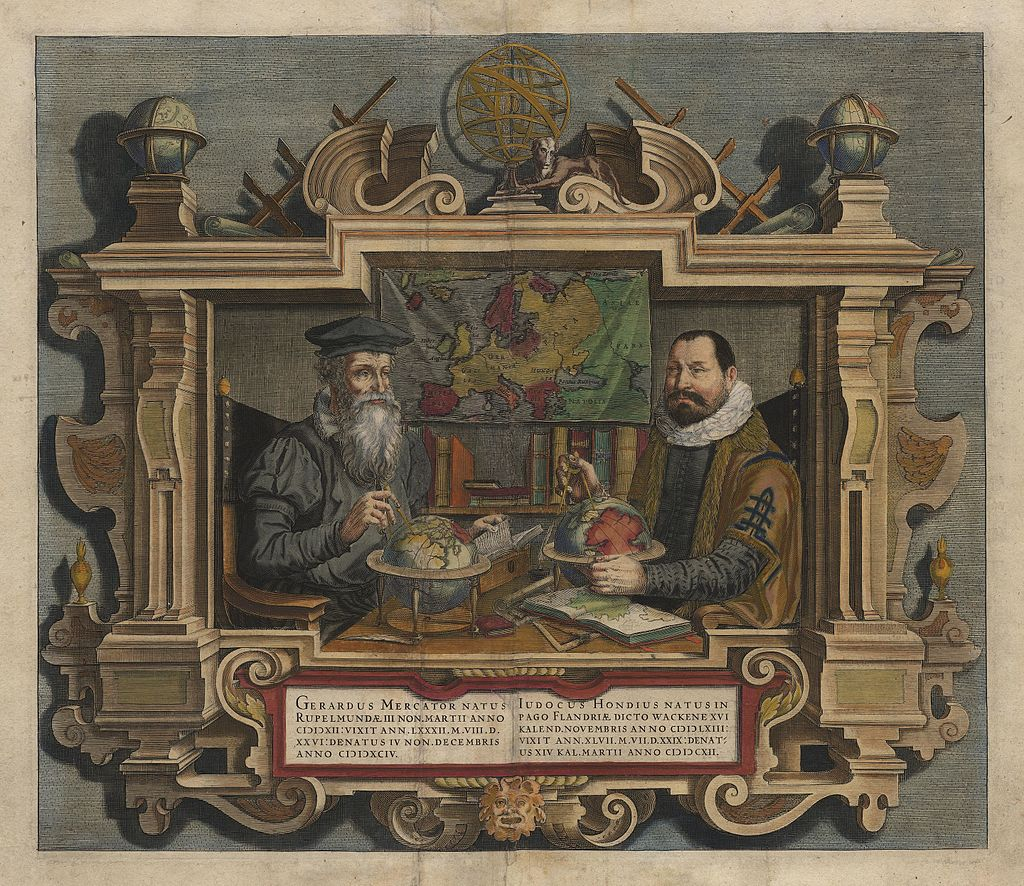
\includegraphics[width=1\linewidth]{../plots/Hondius_Portrait_of_map-makers}
				\caption{Portrait of map-makers, Gerard Mercator and Jodocus Hondius (Jodocus Hondius) source: \url{https://commons.wikimedia.org/wiki/File:Hondius_Portrait_of_map-makers.jpg}}
			\end{figure}
		\end{center}
	\end{column}
	\begin{column}{0.5\linewidth}
		\begin{center}
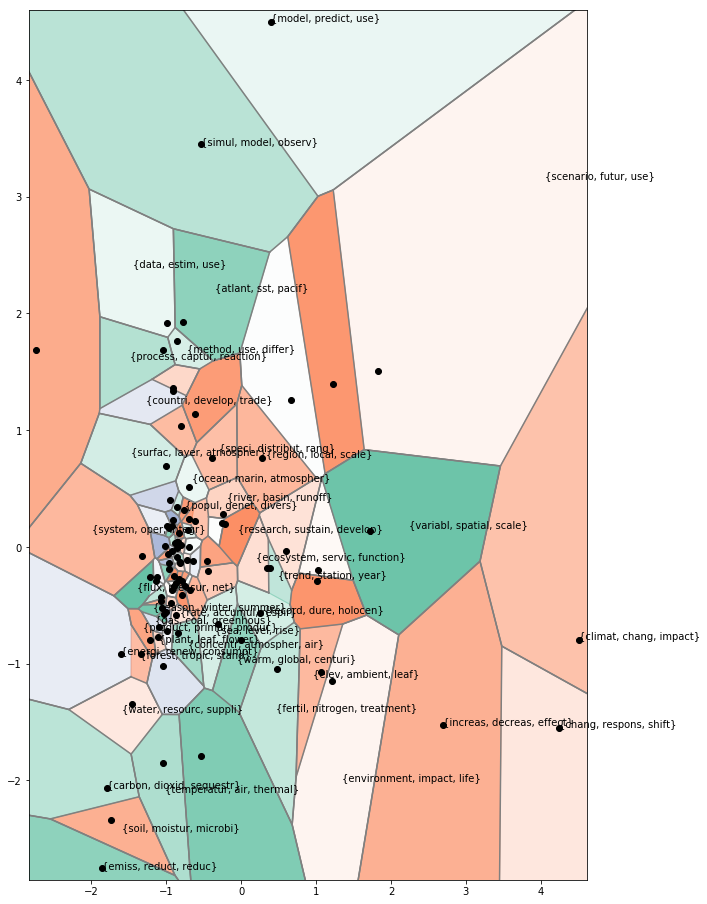
\includegraphics[width=\linewidth]{../plots/pca_map_portrait}
		\end{center}
	\end{column}
\end{columns}
\end{frame}


\begin{frame}{Bibliography}
	\small
	\bibliography{../Mendeley.bib}
\end{frame}

\end{document}
